\documentclass{article}
\usepackage{graphicx}
\usepackage{amsmath}
\usepackage{amssymb}
\usepackage[italicdiff]{physics}
\usepackage{enumerate}
\usepackage{microtype}
\DisableLigatures{encoding= *, family=*}
\usepackage{titlesec}
\usepackage{xfrac}
\setcounter{secnumdepth}{4}
\usepackage{xcolor}
\usepackage[bookmarks=false]{hyperref}
\usepackage{mathtools}
\usepackage{tikz} 
\newcommand*\fullcirc[1][0.3ex]{\tikz\fill (0,0) circle (#1);} 
\usepackage{bigints}
\hypersetup{
    colorlinks=true,
    linkcolor=[RGB]{59 108 209},
    urlcolor=[RGB]{59 108 209}
}
\urlstyle{same}

\titleformat{\paragraph}
{\normalfont\normalsize\bfseries}{\theparagraph}{1em}{}
\titlespacing*{\paragraph}
{0pt}{3.25ex plus 1ex minus .2ex}{1.5ex plus .2ex}

\title{Electrophilic Addition Reaction}
\author{}
\date{}

\begin{document}
\maketitle

\section{Reaction and Mechanism}
\begin{center}
    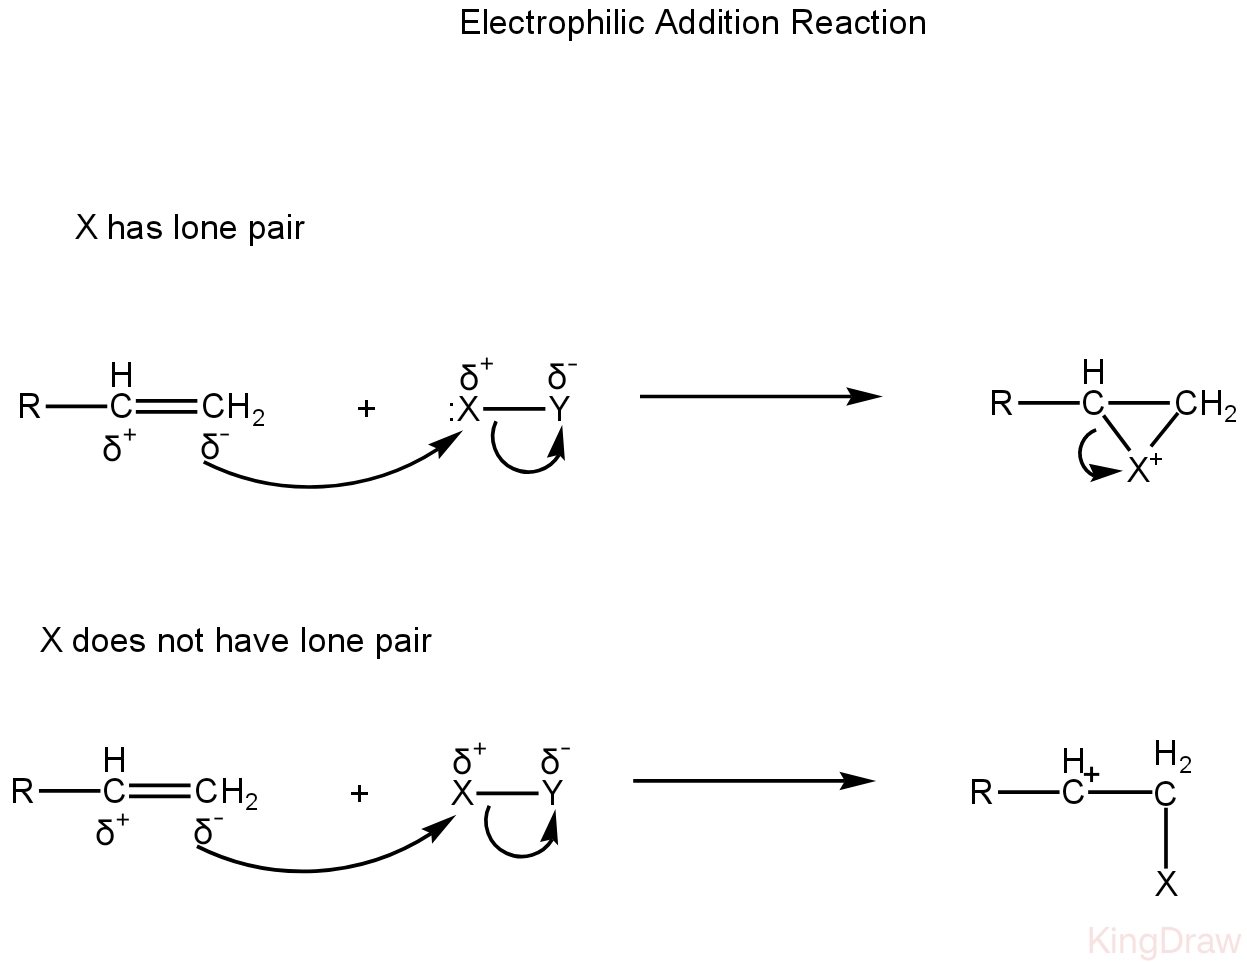
\includegraphics[scale=0.3]{ElectrophilicAdditionReaction_1722210371705.JPEG}
\end{center}
\section{Reaction Observations}
\subsection{$X$ doesn't have lone pair}
\begin{enumerate}[i.]
    \item $C^+$ obtained as intermediate.
    \item Rearrangement can occur.
\end{enumerate}
\subsection{$X$ has lone pair}
\begin{enumerate}[i.]
    \item Non Classical Carbocation (NCC or Cyclohalonium ion) obtained as intermediate.
    \item No Rearrangement.
\end{enumerate}
\section{Reagent Table}

\begin{tabular}{|c| c| c| c| }
    \hline
    Reagent                                         & $E^+$  & $Nu^-$             & Path                   \\[1mm]
    \hline
    $HCl, HBr, HI$                                  & $H^+$  & $Cl^-, Br^-, I^-$  & $X$ does not lone pair \\
    $DCl$                                           & $D^+$  & $Cl^-$             & $X$ does not lone pair \\
    $H^+/H_{2}O, H_{3}O^+, \text{dil.} H_{2}SO_{4}$ & $H^+$  & $OH^-$             & $X$ does not lone pair \\
    $ROH/H^+$                                       & $H^+$  & $OR^-$             & $X$ does not lone pair \\
    $RCOOH/H^+$                                     & $H^+$  & $RCOO^-$           & $X$ does not lone pair \\
    \hline
    $X_{2}/CCl_{4}$                                 & $X^+$  & $X^-$              & $X$ has lone pair      \\
    $Br_{2}/H_{2}O$ or $HOBr$                       & $Br^+$ & $Br^-, OH^-$       & $X$ has lone pair      \\
    $Br_{2}/H_{2}O$ in Brine                        & $Br^+$ & $Br^-, OH^-, Cl^-$ & $X$ has lone pair      \\
    $NOCl$ (Tilden Reagent)                         & $NO^+$ & $Cl^-$             & $X$ has lone pair      \\
    $IN_{3}$                                        & $I^+$  & $N_{3}^-$          & $X$ has lone pair      \\
    \hline
\end{tabular}

\section{KCP and TCP}
\begin{center}
    \begin{tabular}{c | c}
        KCP                                                 & TCP                                  \\
        Kinetically Controlled Product                      & Thermodynamically Controlled Product \\
        $1,2-$ Product is assumed to be KCP                 & Can be $1,2 $ and $1,4$              \\
        Fast Rate                                           & Stable Product                       \\
        Favors at low temperature ($-80, -40, 0 ^ \circ C$) & Favors high temperature
    \end{tabular}
\end{center}
\end{document}